\section{Kosarajus algoritme (Finne SCC)}
Vi kan finne SCCer i en graf $ G $ ved å utføre to dfs. Et på $ G $ og et på $ G^t $, som er grafen vi får ved å snu alle kantene i $ G $. Denne algoritmen kalles Kosarajus algoritme.

\begin{theorem} Kosarajus algoritme

La $ G $ være en rettet graf. Utfør et dfs på $ G $ fra en hvilken som helst startnode, og lagre postfix-telleren (det som ble kalt \mono{highNum} i kodeekempelet i \ref{dfs}). Hvis søket slutter før alle nodene er besøkt, starter vi fra en ny, ubesøkt node.

Snu alle kantene i (transponer) $ G $ og dann $ G^t $. Sorter nodene i $ G $ synkende etter verdien på postfix-telleren. Start et dfs i $ G^t $ fra den noden som har høyest verdi. Alle nodene vi da besøker danner en SCC. Fjern så alle nodene vi besøkte fra grafen $ G^t $, og utfør et nytt dfs fra den noden som nå har høyest tellerverdi. Fortsett slik til alle nodene er besøkt. 
\end{theorem}


\noindent Vi ser på et eksempel:

\begin{example} Finn alle SCCer i grafen:

\begin{figure}[h!]
\centering
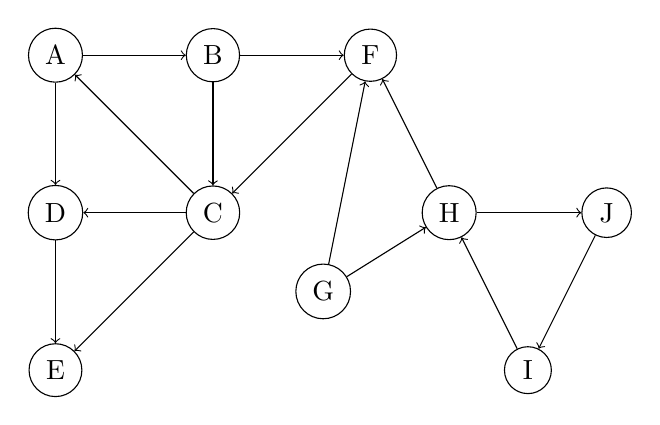
\begin{tikzpicture}[->, align=center]
\tikzstyle{v} = [circle, draw=black]
\tikzstyle{e} = [draw=black]

\node[v] (A) at (-2, 2) {A};
\node[v] (B) at (0, 2) {B};
\node[v] (C) at (0, 0) {C};
\node[v] (D) at (-2, 0) {D};
\node[v] (E) at (-2, -2) {E};
\node[v] (F) at (2, 2) {F};
\node[v] (G) at (1.4, -1) {G};
\node[v] (H) at (3, 0) {H};
\node[v] (I) at (4, -2) {I};
\node[v] (J) at (5, 0) {J};

\draw[e] (A) to (B);
\draw[e] (A) to (D);
\draw[e] (B) to (C);
\draw[e] (B) to (F);
\draw[e] (C) to (A);
\draw[e] (C) to (D);
\draw[e] (C) to (E);
\draw[e] (D) to (E);
\draw[e] (F) to (C);
\draw[e] (G) to (F);
\draw[e] (G) to (H);
\draw[e] (H) to (F);
\draw[e] (H) to (J);
\draw[e] (I) to (H);
\draw[e] (J) to (I);
\end{tikzpicture}
\end{figure}

Vi begynner med å gjøre et dfs. Vi starter i A. Søket stopper etter å ha besøkt A, B, C, D, E og F, og må starte på nytt i G. Startpunktene er valg tilfeldig, og kunne like gjerne vært noen andre. 

\begin{figure}[h!]
\centering
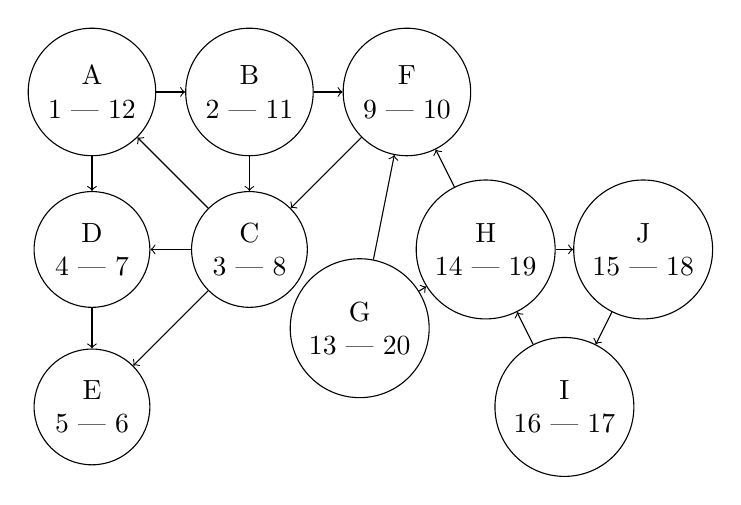
\begin{tikzpicture}[->, align=center]
\tikzstyle{v} = [circle, draw=black]
\tikzstyle{e} = [draw=black]

\node[v] (A) at (-2, 2) {A\\1 | 12};
\node[v] (B) at (0, 2) {B\\2 | 11};
\node[v] (C) at (0, 0) {C\\3 | 8};
\node[v] (D) at (-2, 0) {D\\4 | 7};
\node[v] (E) at (-2, -2) {E\\5 | 6};
\node[v] (F) at (2, 2) {F\\9 | 10};
\node[v] (G) at (1.4, -1) {G\\13 | 20};
\node[v] (H) at (3, 0) {H\\14 | 19};
\node[v] (I) at (4, -2) {I\\16 | 17};
\node[v] (J) at (5, 0) {J\\15 | 18};

\draw[e] (A) to (B);
\draw[e] (A) to (D);
\draw[e] (B) to (C);
\draw[e] (B) to (F);
\draw[e] (C) to (A);
\draw[e] (C) to (D);
\draw[e] (C) to (E);
\draw[e] (D) to (E);
\draw[e] (F) to (C);
\draw[e] (G) to (F);
\draw[e] (G) to (H);
\draw[e] (H) to (F);
\draw[e] (H) to (J);
\draw[e] (I) to (H);
\draw[e] (J) to (I);
\end{tikzpicture}
\end{figure}

\noindent Det hadde vært nok å bare lagre postfixverdiene, men vi har tatt med begge for oversiktens skyld. Vi transponerer $ G $:

\begin{figure}[h!]
\centering
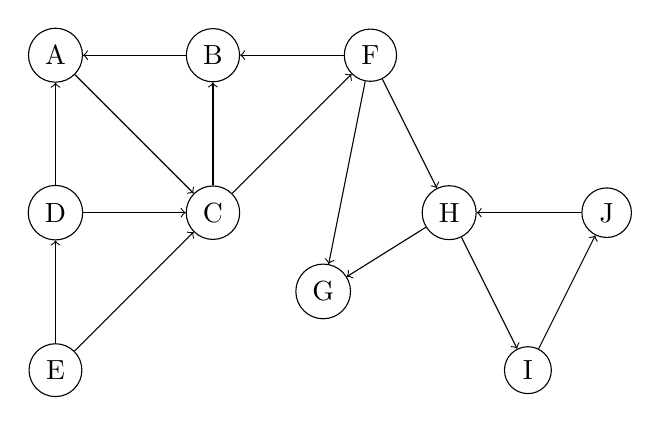
\begin{tikzpicture}[->, align=center]
\tikzstyle{v} = [circle, draw=black]
\tikzstyle{e} = [draw=black]

\node[v] (A) at (-2, 2) {A};
\node[v] (B) at (0, 2) {B};
\node[v] (C) at (0, 0) {C};
\node[v] (D) at (-2, 0) {D};
\node[v] (E) at (-2, -2) {E};
\node[v] (F) at (2, 2) {F};
\node[v] (G) at (1.4, -1) {G};
\node[v] (H) at (3, 0) {H};
\node[v] (I) at (4, -2) {I};
\node[v] (J) at (5, 0) {J};

\draw[e] (B) to (A);
\draw[e] (D) to (A);
\draw[e] (C) to (B);
\draw[e] (F) to (B);
\draw[e] (A) to (C);
\draw[e] (D) to (C);
\draw[e] (E) to (C);
\draw[e] (E) to (D);
\draw[e] (C) to (F);
\draw[e] (F) to (G);
\draw[e] (H) to (G);
\draw[e] (F) to (H);
\draw[e] (J) to (H);
\draw[e] (H) to (I);
\draw[e] (I) to (J);
\end{tikzpicture}
\end{figure}

Siden G har høyest postfixteller (20) begynner vi der. Vi ser i $ G^t $ at G ikke har noen kanter ut. Første SCC er derfor \{G\}. Når vi tar vekk G fra grafen er det H som har høyest postfixverdi (19), vi starter derfor neste dfs derfra. Vi går fra H til I og J, før vi treffer på H igjen. Vi går tilbake, men siden hverken J eller I har flere etterfølgere stopper søket, og neste SCC er derfor \{H, I, J\}. Nå er det A som har høyest postfixteller (12), så vi starter derfra. Fra A går vi til C, og til B. Da møter vi på A igjen, så vi går tilbake til C og videre til F. Vi går \emph{ikke} fra F til G eller H, siden de allerede er besøkt tidligere. Vi går derfor tilbake til C og tilbake til A. I det søke besøkte vi \{A, B, C, F\}, det blir derfor neste SCC. Til slutt starter vi i D (7), men siden D ikke har noen kanter til ubesøkte noder stopper søket med en gang. Det samme skjer i E (6). 

Alle SCCer til $ G $ er: \{ \{G\}, \{H, I, J\}, \{A, B, C, F\}, \{D\}, \{E\} \}
\end{example}

\noindent Det finnes en forbedring av denne algoritmen som bare bruker ett DFS. Søk opp \textit{Tarjans algoritme}

\subsection{Kompleksitet}
Vi ser at vi må gjøre to DFS, og en transponering. DFS besøker alle noder og alle kanter én gang, og går derfor i $ O(\abs{V} + \abs{E}) $. Transponering må besøke alle kantene én gang, og går derfor i $ O(\abs{E}) $ tid. Tilsammen har Kosarajus algoritme $ O(\abs{V} + \abs{E}) $.